\lecture{7}{Mon 20 Jan 2020 16:28}{}

Last Time:
\begin{itemize}
	\item Linear inhomogeneous equations
		\begin{enumerate}
			\item Nonautonomous (constant coefficient)
				\begin{align*}
					\hat{F}\left( t, x \right)  &=  A\left( t \right) x \\
					\dot{\xi} \left( t \right) &= A\left( t \right) \xi\left( t \right) \\
					\Phi ^{\hat{F}}\left( t, t_0, x_0 \right) &= \Phi_{A}\left( t, t_0 \right) x_0 
				.\end{align*}
			\item Autonomous (constant coefficient)
				\begin{align*}
					\hat{F}\left( t, x \right)  &=  A x \\
					\dot{\xi}  &= A \xi \\
					\Phi ^{\hat{F}}\left( t, t_0, x_0 \right) &= e^{A\left( t - t_0 \right) }x_0
				.\end{align*}
		\end{enumerate}
\end{itemize}

\subsection{Linear Inhomogeneous Equations (Summary)}
\subsubsection{Non constant coefficient case}

\begin{align*}
	\hat{F}\left( t, x \right) &=  A\left( t \right) x + f\left( t \right) , \quad f \in  L'_{loc}\left( \T; X \right)  \\
	\dot{\xi} \left( t \right)  &=  A\left( t \right) x + f\left( t \right)  \\
	\Phi^{\hat{F}}\left( t, t_0, x_0 \right)  &= \Phi_{A}\left( t, t_0 \right) x_0 + \int_{t_0}^{t} \Phi_{A} \left( t, \tau \right) f\left( \tau \right) d\tau 
.\end{align*}

\subsubsection{Constant Coefficient Case}
\begin{align*}
	\hat{F}\left( t, x \right) &=  A x + f\left( t \right) , \quad f \in  L'_{loc}\left( \T; X \right)  \\
	\dot{\xi} \left( t \right)  &=  A\xi\left( t \right) x + f\left( t \right)  \\
	\Phi^{\hat{F}}\left( t, t_0, x_0 \right)  &= e^{A\left( t - t_0 \right)} x_0 + \int_{t_0}^{t} e^{A \left( t - \tau \right)} f\left( \tau \right) d\tau 
.\end{align*}

This is known as the "variation of constants" formula.

\section{Distributions}
Let's think back to a distribution from an earlier course:
\begin{figure}[htpb]
	\centering
	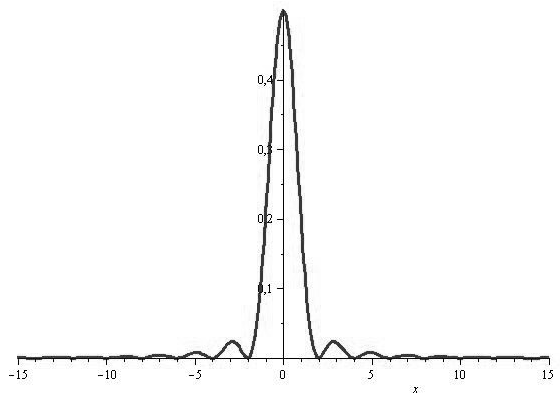
\includegraphics[width=0.8\textwidth]{./figures/Fejer-kernel.png}
	\caption{The Fejer Kernel}
	\label{fig:}
\end{figure}

This distribution converged to infinity at $x = 0$ and 0 everywhere else, as $n \to \infty$. 

\begin{example}
	Simple ODE: $\dot{\eta} \left( t \right)  = \mu_{j}\left( t \right) $, $\eta\left( 0 \right)  = 0$.
	\[
		\mu_{j}\left( t \right) = \begin{cases}
			j & t \in  \left[ 0, \frac{1}{j} \right] \\
			0 & \text{ otherwise}
		\end{cases}
	.\] 
	Solve for $\eta_{j}$ with input $\mu_{j}$ :
	\begin{align*}
		\mu_{j}\left( t \right) &= \begin{cases}
			\int_{0}^{t} jd\tau & t \in \left[ 0, \frac{1}{j} \right]  \\
			\int_{0}^{\infty} \mu_{j}\left( \tau \right) d\tau & t \in \left( \frac{1}{j}, \infty \right) 
		\end{cases}
		\implies \eta_{j}\left( t \right) &= \begin{cases}
			jt & t \in  \left[ 0,\frac{1}{j} \right]  \\
			1 & t \in \left( \frac{1}{j}, \infty \right) 
		\end{cases}
	.\end{align*}

	As $j \to  \infty$,
	\begin{align*}
		\lim_{j \to \infty} \mu_{j}\left( t \right) &= \begin{cases}
			\infty & t = 0\\
			0 & \text{ otherwise}
		\end{cases} \\
		\lim_{j \to \infty} \eta_{j} \left( t \right) &= \begin{cases}
			1 & t \in  \left( 0, \infty \right) \\
			0 & \text{ otherwise}
		\end{cases} \\
			&= \eta_{\infty}\left( t \right) 
	.\end{align*}
\end{example}
 
$\eta_{j}$ is the output for input $\mu_{j}$. Is $\eta_{\infty}$ the output for input $\mu_{\infty}$? NO.

Is there an input which gives $\eta_{\infty}$ as an output? NO. We will see later why. 

Can we enlarge what we consider as inputs from locally integrable to something else? YES, distributions!

\section{Test Functions}

\begin{definition}[Test Functions]
	Denote by $D\left( \R, \F \right) $ the set of $\infty$-ly differentiable functions with compact support. IE, $D\left( \R; \F \right) = C^{\infty}_{cpt}\left( \R; \F \right) $. Elements of $D\left( \R; \F \right) $ are test functions. 
\end{definition}

\begin{example}
	\begin{enumerate}
		\item $\Phi\left( t \right) = 0 \forall  t $ is in $D\left( \R;\F \right) $.
		\item Are there nonzero elements of $D\left( \R; \F \right) $?
			
	\end{enumerate}
\begin{figure}[ht]
    \centering
    \incfig{test-function}
    \caption{test function}
    \label{fig:test-function}
\end{figure}

The equation
\[
	\frac{d}{dt} = \frac{1}{P\left( t \right) } e ^{-\frac{1}{1 - t^2}}
.\] 	
is an example of a nonzero element if $D\left( \R;\F \right) $. 
\end{example}

\begin{definition}
	A sequence $\left( \varphi_{j} \right) _{j \in \Z_{>0}}$ converges in $D\left( \R; \F \right) $ to zero if 
	\begin{enumerate}
		\item $\exists K \subseteq \R $ compact such that $supp\left( \varphi_{j} \right) \subseteq K$ for $j \in  \Z_{>0}$. 
		\item $\left( \varphi_{j}^{\left( k \right) } \right) _{j \in  \Z _{>0}}$ converges uniformly to zero for every $k \in  \Z_{\ge 0}$, ie, $\varphi_{j}$ and all of its derivatives converge uniformly. 
	\end{enumerate}
\end{definition}
